\section{Distributed Systems}

    The MARS cloud is architectured as a distributed system. Thus, it is of great importance to understand
    this architecture, so that one can anticipate the operations of the MARS framework and
    the technical challenges that could occur due to its complex structure.
    \par
    A distributed system can be defined as a number of autonomous computing elements which 
    appear to a user as a single coherent system \cite[p.~2]{DistributedSystems}. This definition implies that the system is split into meaningful domains which behave 
    independently from each other and that the system supports resource sharing in order to appear as single coherent application to the user. 
    For the system to appear as a single coherent system the individual units must establish some kind of collaboration
    with each other usually done by exchanging messages over a network. This enables the system to share different resources that are physically separated, 
    as an element in the system can be controlled by passing messages.


    %These individual elements mentioned could be either a hardware device or possibly a software process known as nodes. A node can
    %be classified from a very high-performance computers with lots of processing power to a simple and cheap computer owned by an average individual. 
    %In practice, the nodes must communicate with one another via exchanging messages to achieve certain objective \cite[p.~2]{DistributedSystems}.
    

    \begin{figure}[H]
        \centering 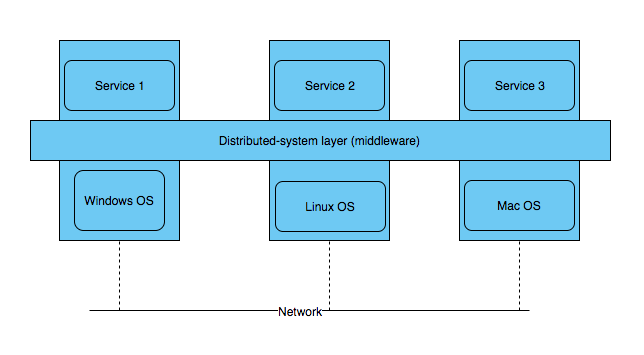
\includegraphics[scale=0.5]{grafiken/distributedSystem.png}
        \caption{A distributed system extended over multiple devices with same application 
        interface \cite[p.~5]{DistributedSystems}}
        \label{fig:distributedSystem}
    \end{figure}

    \par
    Distributed Systems can be utilized to realize a complex application dispersed across
    multiple machines which communicates via a network protocols (e.g. HTTP \cite{HTTP}, 
    GRPC \cite{grpc}). The 
    components interact with each other to achieve a common goal. It also provides
    more reliability compared to a non-distributed system because there is no single point
    of failure when a system is designed properly. 

    \par
    Figure \ref{fig:distributedSystem} shows an example of an application being 
    distributed amongst different computers. It can also be seen that the different parts of the application are allowed
    to communicate via a common middleware whose main responsibility is to
    efficiently manage resources across the distributed applications. This kind of system
    makes most sense for deployment which require high performance computing power as this system can allow an application to share different
    resources (e.g CPU power, memory and storage) located in another machine.



    
        
    \subsection{Advantages of a Distributed System} 
        \subsubsection{Reliability and Availability}
        One of the main reasons for building a distributed system is to make the application free from single failure events.
        Since the application is generally spread across different nodes connected via a network, failure of a single node will not 
        crash the system completely. This makes a distributed system more available, reliable, and independent to a user as the availability
        of the application is not hindered completely.
        
        \subsubsection{Scalability}
        Scalability is an important step in software development process, as the requirements for an application tends to changes by time and also requires more resources
        (e.g. more processing power, more data volume). 
        In contrast to a single system, where the computer 
        has to be replaced completely by a really high end device, there is a possibility to just expand the system but adding another device in the network.
        Since the application in a distributed system are able to communicate via network it is easier to scale and add more resources and 
        also scale down if required. 
    
    \subsection{Challenges}    
        \label{subsection: distriChallenges}
        \subsubsection{Data Coherency}
        The data is said to be coherent when it is uniform across an entire network. In other words, data is coherent when all
        the resources between a server and a client is synchronized. 
        Since a distributed system is susceptible to network failures, a network partition \cite[p.~59]{CAP} cannot be avoided. In presence
        of a network partition the change in data will not be synchronized to all of its client leading to have inconsistent data. Furthermore, the
        complexity to maintain this coherency increases drastically when the system has more clients trying to gain access to the data. This phenomena
        must be taken into consideration while designing an application for this kind of system.

        \subsubsection{Network Issues}
        Generally in a distributed system, different applications communicate via network protocols i.e. HTTP, GRPC. It is to be noted that
        communication via a network is not always reliable. This is because managing a distributed network is rather complex. Also due to
        external reasons the communication can break leading to loss of messages which disables some parts of the application. 
        This phenomena is also not seen in a single system.

        \subsubsection{Error Handling}
        Errors are imminent in every application and to continue working normally again it has to detect and recover from them.
        Detecting errors in a distributed system requires a different approach since the application is spread across multiple systems. 
        It is not enough that each service ensures its own correctness because the system is interconnected via a
        network connection. Due to the fact that the network is also involved in a distributed system there are additional error detection methods that have
        to be implemented. This brings up more complications in comparison to a single system where an error is contained within a single system.

         
